\documentclass[10pt,journal,compsoc]{IEEEtran}


% *** CITATION PACKAGES ***
%
\ifCLASSOPTIONcompsoc

  \usepackage[nocompress]{cite}
\else
  % normal IEEE
  \usepackage{cite}
\fi

% *** GRAPHICS RELATED PACKAGES ***
%
\ifCLASSINFOpdf
  \usepackage{graphicx}
  % declare the path(s) where your graphic files are
  \graphicspath{{Figures/}{Other_Folder/}}
  % and their extensions so you won't have to specify these with
  % every instance of \includegraphics
  \DeclareGraphicsExtensions{.pdf,.jpeg,.png}
\else

\fi
% *** SUBFIGURE PACKAGES ***
\ifCLASSOPTIONcompsoc
 \usepackage[caption=false,font=footnotesize,labelfont=sf,textfont=sf]{subfig}
\else
 \usepackage[caption=false,font=footnotesize]{subfig}
\fi

\usepackage{url}
\usepackage{hyperref}




\hyphenation{op-tical net-works semi-conduc-tor}


\begin{document}

\title{Implementation and Performance\\Analysis of a Parallelized Solution for\\{\itshape Storms of High-energy Particles}}

\author{Gonçalo~Moura,~\IEEEmembership{Student,~52361,}
        Gonçalo~Querido,~\IEEEmembership{Student,~45616,}
        and~Renato~Oliveira,~\IEEEmembership{Student,~52393}
        
\IEEEcompsocitemizethanks{\IEEEcompsocthanksitem All three students were enrolled at NOVA School of Science and Technology, Department of Computer Science.\protect\\
E-mails: gb.moura@campus.fct.unl.pt; gq.sousa@campus.fct.unl.pt; rjs.oliveira@campus.fct.unl.pt
}% <-this % stops an unwanted space
}



% The paper headers
\markboth{Concurrency and Parallelism, June~2021}%
{Shell \MakeLowercase{\textit{et al.}}: Bare Demo of IEEEtran.cls for Computer Society Journals}

\IEEEtitleabstractindextext{%
\begin{abstract}
In this report we will approach topics regarding the parallelization of a problem concerning a programming code that simulates high-energy particles bombardment on a surface. Through a given code, this report is focused on analysing the effect of the speed up and accuracy of a parallelized code compared to its sequential version, using the application programming interface {\itshape OpenMP}, that allows for a multithreading implementation, and using the {\itshape Instruments} Profiler to measure memory/resource usage during the execution to evaluate where better to act. To overcome the parallelization problems found, the solution will be based on the slides given to us on the theoretical and practical classes, having always in regard the bibliography suggested for study. \cite{Conc} \cite{Paral}
\end{abstract}
}


% make the title area
\maketitle

\IEEEdisplaynontitleabstractindextext

\IEEEpeerreviewmaketitle

\IEEEraisesectionheading{\section{Introduction}\label{sec:introduction}}

\IEEEPARstart{T}{his} report will be focused on the implementation of a possible parallelized solution regarding the problem of {\itshape Storms of High-energy Particles}. This solution will be used to compare and analyze performance and speed-up results against its sequential version.
\\During the report, every bit of code that was thought to be beneficial to be parallelized will be discussed, giving a theoretical context on why it was decided, supported by tested results. We will discuss the implementation strategy as well as all the problems had in its execution. To measure the amount of resources used and to analyze the code {\itshape hotspots}, we resorted to a {\itshape profiler}, and in this report we chose {\itshape Instruments} for {\itshape MAC OS} for this purpose. Due to running errors later encountered, our results from comparing the sequential version to the pararellized one were measured from a machine with {\itshape Linux OS}.
\\The {\itshape OpenMP} API (aplication programming interface) was used for this implementation as specified in the project requirements, allowing for a simple and flexible interface for programs that require parallelism within a multi-core node, allowing for an implementation of multithreading. 
\\To proceed to a proper analysis, assuring there are as fewer changes as possible, all tests were run in the same machine. Most of them were run forty times using each solution (forty times the sequential code and forty times the parallelized code) while others, more specifically tests seven, eight and nine, were only run twenty-five times due to their bigger execution runtime. The results discussion will be based around test seven due to it being big enough to compare possible solutions. 

\section{OpenMP API}

{\itshape OpenMP} is a parallel programming model for multiprocessor architectures, providing a portable and scalable model for developers of shared memory parallel applications. It allows programmers to set the maximum number of threads a program can create to run in parallel within the bit of code that is marked accordingly, running that section independently.\cite{OpenMP} At the end, the threads then join back into the primary one, continuing to the end of the program.
\\It gives access to an extensive library specialized in dealing with threads for parallelization purposes.

\begin{figure}[b]
    \centering
    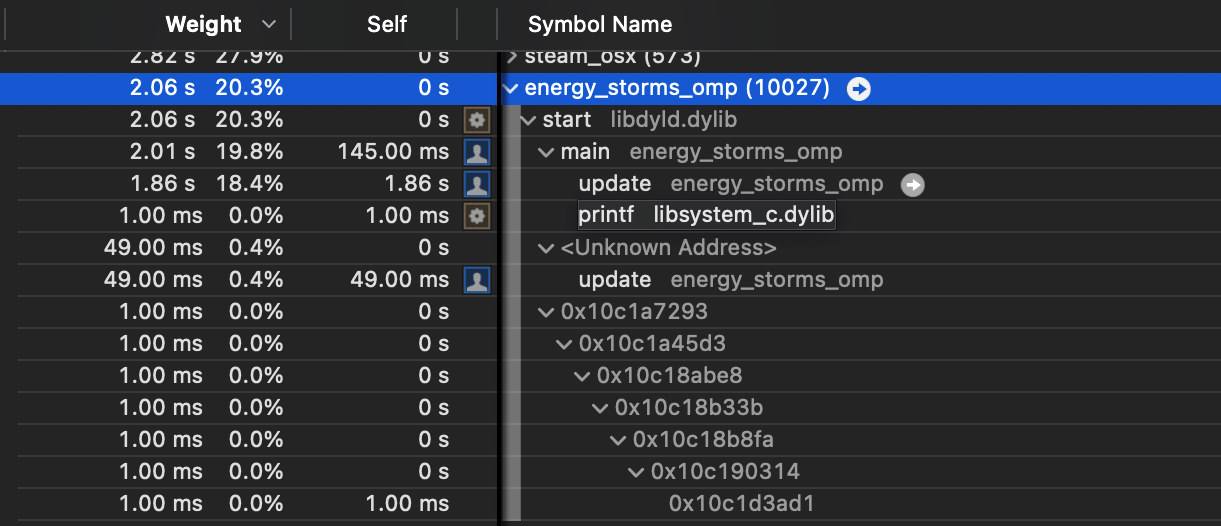
\includegraphics[scale=0.4]{profiler_data.png}
    \caption{\itshape{Output of the Profiler Instruments after the first excecution}}
    \label{fig:my_label}
\end{figure}

\section{Profiler}

In order to discover CPU activity variation and memory allocation for each step of the code, we used a profiler to display the events occurring in the application. The one chosen to discover what was needed was {\itshape Instruments} (formerly known as {\itshape Xray}), for {\itshape MAC OS}.\cite{Prof}
\\By using this profiler, we discovered that, by running the {\itshape .omp} file, it uses 20.3 percent of the computer processor. On the same information, we can see that the update function present in the given code takes 18.4 percent, as seen in {\itshape Fig. 1}. By doing the math, we can conclude that the update function ends up weighting as much as 90.64 percent on the processor.
\\With this information, we can conclude that most of the processing power goes to the {\itshape update} function. With this information, we can claim that this function is a discovered {\itshape hotspot}, so it his in our interest to parallelize the parts of the code that invoke this function in order the improve the execution performance.

\begin{figure}[b]
    \centering
    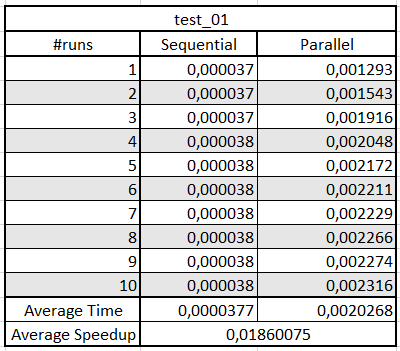
\includegraphics[scale=0.5]{test1_results.png}
    \caption{\itshape{Time and speed up results upon running the Test 1 sequentially and parallelized with sixteen threads running.}}
    \label{fig:test1}
\end{figure}

\section{Parallelized Code}

In this section we will talk about the parts of the code we thought would improve performance by applying parallelization, as present in the {\itshape .omp} file, referencing the sections by the name of the method and the number of the block in that method (if there is one, if not it will be specified by the line number).
\\As discussed before, we were able to find the {\itshape hotspot} through the analysis of profiler's result, and therefore we want to try to parallelize all the situations where the function {\itshape update} is invoked and check for results and possible improvements on performance.

\subsection{Parallelizing the {\itshape update} Function}

A simple parallelization was aplied to the function {\itshape for} cycle, using, as mentioned before, the {\itshape OpenMP} library. After this implementation we proceeded in analysing the next blocks of code to see if it was worth to parallelize. For example, we analyzed block 4.2, that updates the arrays {\itshape layer} and {\itshape layer\_copy} using basic operations, not being necessary to apply a parallelization.

\subsection{Block 4.3}

By analysing this block, we came across a considerable problem: by applying parallelization on this section and updating the values, they were being printed with incorrect values. This happened due to the fact that several threads were trying to access the same position of the vector, and changing the same value each time a thread accessed one position. To overcome this issue, three different approaches were tried: 
\begin{itemize}
  \item using the sequential function;
  \item using the {\itshape atomic} function from the {\itshape OpenMP} library;
  \item using the {\itshape critical} function also from the {\itshape OpenMP} library.
\end{itemize}

\subsubsection{Sequential Function}
Although it is not an implemented solution, it is important to analyse the performance and speed up values the sequential version can produce.
\\As seen on {\itshape{Fig. 2}}, when running the code using the test file {\itshape test\_01}, the sequential version has a considerable lower average time of execution when compared to its parallel counterpart, having no speedup at all. 
\\Although one might assume that if this happened with this test case, then a sequential version of the code might be better than any form of parallelization for this problem. However, we need to have in consideration the size of the test case. {\itshape test\_01} is very small compared to a real situation, or even the other test cases, so it cannot serve as a reference. It is only safe to say that, for an array with so few positions filled, it is not worth to parallelize on this problem.

\subsubsection{{\itshape Atomic} Function}
The usage of {\itshape OpenMP's} atomic operation allows a multiple threads to update a shared numeric variable.\cite{OpenFull}
\\At first this implementation was slightly faster than the other two enumerated, and was decided to keep it parallelized with this function. Although, after running several test using a different number of threads, we arrived at the conclusion that it was not a viable solution, because, as happened in the initial try, some values were being returned incorrectly. This could be because of the fact that the {\itshape atomic} function only just be able to perform atomic operations to update variables, conflicting with the verification to determine the maximum of the array of values. 

\subsubsection{{\itshape Critical} Function}
Using {\itshape OpenMP's} critical function allows to set a section of the code as critical, meaning that only one thread at a time can enter that bit. Only when a thread is finished running the delimited section, can the next thread run it.\cite{OpenFull}
\\Compared to the atomic implementation, by being able to synchronize the access to blocks by different threads, the accuracy errors discovered above mentioned were solved, at the cost of decreased performance.

\begin{figure}
    \centering
    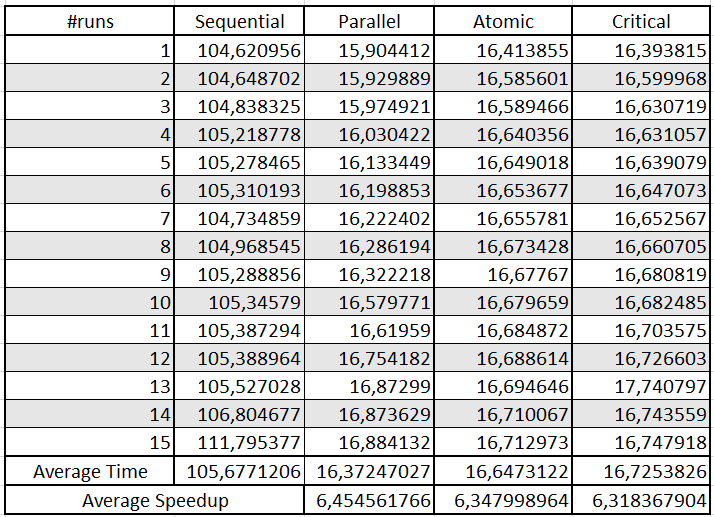
\includegraphics[scale=0.35]{test7_results.png}
    \caption{\itshape{ Results obtained by running test\_07 fifteen times using all four possible solutions.}}
    \label{fig:my_label}
\end{figure}

\subsection{Result comparison}

After implementing the best found solution, resorting to {\itshape OpenMP's} critical operation, maintaining the needed accuracy, we proceeded to run the tests with different numbers of threads. To analyse the values in the best way possible, we run the the code with two, four, eight, sixteen and eighteen threads.
\\In {\itshape Fig. 3} we present the results obtained by running {\itshape test\_07} with sixteen threads using the sequential, parallel (with simple {\itshape .omp} techniques), {\itshape Atomic} and {\itshape Critical} functions. To facilitate the result's presentation, of the forty tests run only the first fifteen are shown. We can interpret that either the {\itshape atomic} solution or the {\itshape critical} promising, whereas the parallel perform worse. Even though the parallel version has a promising start, its execution time increases considerably with each iteration, worsening test after test. 
\\Looking at {\itshape Fig. 4}, we can observe the final results of running the {\itshape test\_07} using all four solutions. Here we can see that the solution with highest speedup and the best average time after the forty tests is the one using the {\itshape atomic} approach, although, as discussed in a previous topic, it fails in accuracy. On the other hand, the {\itshape critical} approach has nearly one hundred per cent accuracy, and the cost of performance versus accuracy is something we can bear, as the performance and average speedup is very similar.
\\Regarding the number of threads and how it affects performance, we can conclude by looking at {\itshape Fig. 5} that, as we increase the number of threads, the execution time of our program decreased. We can observe this phenomenon happen on up to sixteen threads. After this number, the execution time starts rising, being the performance cap at sixteen threads.
\\We associate this behaviour to the fact that the machine used to run the tests was running on a {\itshape WSL} environment, enabling to run native {\itshape Linux} command-line tools directly on Windows. This {\itshape WSL} environment was set to sixteen logical cores, limiting the recognized cores to run this implementation, being consequently limited in terms of efficiency to sixteen threads.

\begin{figure}
    \centering
    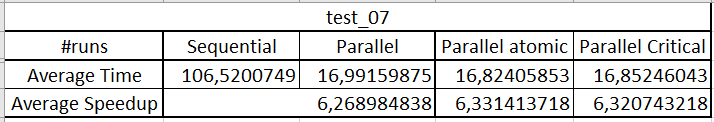
\includegraphics[scale=0.35]{test_07_final.png}
    \caption{\itshape{Final results after running test seven forty times}}
    \label{fig:my_label}
\end{figure}

\begin{figure}
    \centering
    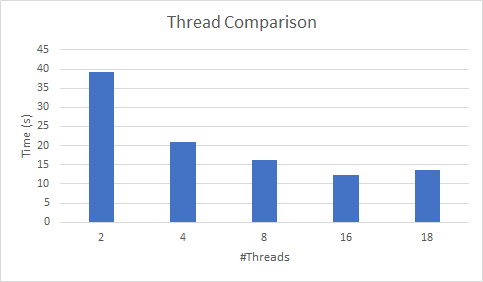
\includegraphics[scale=0.5]{thread_comparison.png}
    \caption{\itshape{Thread comparison while running test\_07 with a parallelized solution.}}
    \label{fig:my_label}
\end{figure}

\section{Cluster}

To provide us with further data to analyze our solution, we ran {\itshape test\_07} with our parallelized solution on the {\itshape cluster} with one wave file, two wave files and three wave files. The performance values returned are present on {\itshape Fig. 6}.
\\By analyzing the data, we can see that the execution times in the {\itshape cluster} compared to the local machine used are considerably different, having a large gap between the average time each of them takes to run each wave.
\\In order to better understand why these values are so apart from each other, we decided to check the {\itshape cluster specifications} and compare them to our local machine. Even though, after checking, we could not conclude anything that would interfere so much with the performance, as the number of {\itshape cores} in the cluster are the same as the local machine.
\\What we suspect might have some impact in these values is the CPU of each machine.

\begin{figure}
    \centering
    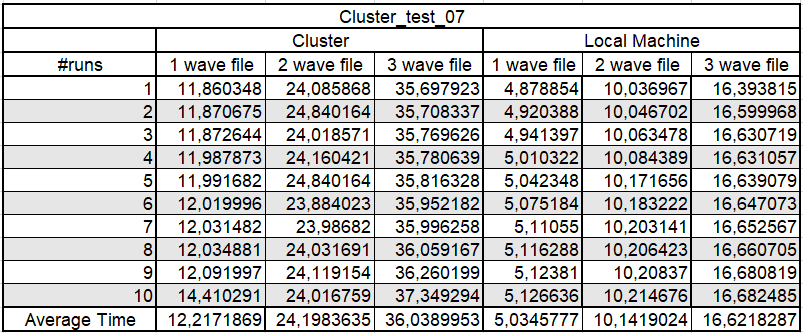
\includegraphics[scale=0.30]{cluster_test_07.png}
    \caption{\itshape{Comparison between cluster and local machine while running test\_07 with a parallelized solution.}}
    \label{fig:my_label}
\end{figure}

\section{Conclusion}
To parallelize a program it is very important to find the {\itshape hotspots} and dependencies present in the code, as it gives us an insight on where to start analyzing. By discovering where most of the processing power goes to, we were certain that, if it could be parallelized, the performance could be improved.
\\According to the results obtained, the parallelization was, in most cases, successful, leading to a decrease in execution time compared to the given sequential version.
\\We believe better results could be obtained by discovering other relevant bits of code where parallelization could be applied. We do not take this as a perfect solution for the whole problem, but as a considerable improvement in situations where large amount of data are present. 

% use section* for acknowledgment
\ifCLASSOPTIONcompsoc
  % The Computer Society usually uses the plural form
  \section*{Acknowledgments}
  
\else
  % regular IEEE prefers the singular form
  \section*{Acknowledgment}
\fi

 We would like to thank Pedro Dimas, student number {\itshape 52919} for providing us with {\itshape script} that allowed us to run a test multiple times. We would also like to thank {\itshape Group 24} for being part of the brainstorming on how to approach this project's parallelization problem.
 
\section*{Individual Contributions}

The work was divided in the following form: Gonçalo Moura was the main responsible for the code parallelization (33\%), helped by Renato Oliveira. Renato was responsible by the testing fase (33\%), helped by Gonçalo Moura, both in his machine and in the cluster. Gonçalo Querido was the main responsible for the report and analysing the data (33\%), where in this last part he was supported by his fellow group members who also gave him the graphs. Since we were able to be physically together it the last days, we do believe we all worked the same amount, helping in everything we could, and so splitting the relative contribution evenly.

\ifCLASSOPTIONcaptionsoff
  \newpage
\fi

\begin{thebibliography}{10}

\bibitem{OpenMP}
R.~Gonçalves, \emph{Paralelização de Aplicações com OpenMP}, Revista PROGRAMAR, 2014.
  
\bibitem{Conc}
M.~Raynal, \emph{Concurrent Programming: Algorithms, Principles, and Foundations}, Springer, 2013.

\bibitem{Paral}
M.~McCool,~A.~Robison and J.~Reinders, \emph{Structured Parallel Programming}, Elsevier, 2012.

\bibitem{Prof}
https://docs.elementscompiler.com/Platforms/Cocoa/Instruments/

\bibitem{OpenFull}
http://portal.nacad.ufrj.br/online/intel/advisor2017/help/index.htm\#GUID-BFE5F55E-A3BD-4440-B285-8FBF6A53A30E.htm

\end{thebibliography}
  
\end{document}


